\documentclass[a4paper]{article}
\usepackage{anysize}
\marginsize{1cm}{1cm}{1cm}{1cm}

\usepackage{amssymb}
\usepackage{amsmath}
\usepackage[pdftex]{graphicx}
\usepackage{epsfig}
\usepackage{subfigure}
\usepackage{listings}
\lstset{language=haskell}
\lstset{commentstyle=\textit}
\lstset{mathescape=true}
\lstset{backgroundcolor=,rulecolor=}
\lstset{basicstyle=\ttfamily}
%\linespread{2.0}

\begin{document}

\title{\bf Monadic Object Encodings}

\author{Giuseppe Maggiore \quad Michele Bugliesi
 \\ Universit\`a Ca' Foscari Venezia
 \\ Dipartimento di Informatica 
 \\ \{maggiore,bugliesi\}@dsi.unive.it
}

\date{}
\maketitle

\begin{abstract}
In this paper we define a model for expressing highly generic
computations with objects in Haskell. Our objects manipulate
some abstract memory. We do so with a twofold objective:
\begin{itemize}
\item to be able to define various, different concrete 
implementations of our objects that implement different
behaviors such as transactional computations, reactive
programming, mutable programs, etc;
\item to be able to perform various kinds of static analysis 
on memory management and computations, thereby having 
type-safe dynamic memory management, type-safe reflection, 
and other similar opportunities.
\end{itemize}
\end{abstract}

\section{Introduction}
\label{sec:intro}
%%%%%%%%%%%%%%%%%%%%%%%%%%%%%%%%%%%%%%%%%%%%%%%%%%%%%%%%%%
% intro.tex
%%%%%%%%%%%%%%%%%%%%%%%%%%%%%%%%%%%%%%%%%%%%%%%%%%%%%%%%%%

Video-games touch many of the fields of computer science. Video-games are heavy in:
\begin{itemize}
\item maths and physics: from the projective algebra and lighting models used in rendering to the physical simulations that make a virtual world feel more ``real"
\item algorithms: we find balanced spatial trees for efficiently querying the world for objects based on a position to pathfinding algorithms for automated navigation of the game environment
\item optimization: games must run fast, or the user loses the feeling of immersion because of stuttering; no CPU cycles should be wasted
\item networking: multiplayer games implement both client-server and peer-to-peer architectures in order to synchronize the game state across a network
\item abstraction: to allow for ``scripting", that is layering custom behaviors on top of the basic architecture, games must support a programmable interface (sometimes with an entire interpreter for an external scripting language)
\end{itemize}
Most games are written in relatively low-level languages such as C/C++. These languages allow the writing of complex applications that can run very fast thanks to the careful hand-crafted management of hardware resources; while this is certainly a good thing, the amount of effort required on the part of programmers is much higher than it could be. In this paper we will discuss the general architecture of a game, and how the various problems encountered when building a small game can be solved.

\subsection{General shape of a game}
A game requires at the very least two functions:
\begin{itemize}
\item an initialization function that starts-up the game by setting its inital state
\item a drawing function that (many times per second, at least at around $20Hz$, to give the illusion of smoothness) updates and re-draws the game state
\end{itemize} 
It is common to split the drawing function in two parts:
\begin{itemize}
\item the updating function that updates the game state
\item the drawing function that re-draws the updated game state
\end{itemize}
This further separation is warranted by the complexity of these operations. Updating can be seen as a step of a numerical integrator: we know the state and its derivative with respect to time, and we compute the next state by ``integrating" it. This view is relatively simplistic, but it gives a clear idea of the role of the update function. Also, because of the nature of the update function, its execution must be very fast: if an update lingers for too long, then draw will not be executed and the smootness of the animations will suffer. Long computations must be manually split over various updates.
Drawing is also a complex operation. Usually it involves visibility determinations to avoid rendering parts of the scene that will not be visible on screen, either due to occlusions or because it is outside of the viewing frustum.

The problems we will tackle in this paper are mostly associated with the architecture of a game. We will start by showing how we would build a game in a purely imperative fashion in the C\# language. Our implementation is very straightforward and could have been easily done in C++. This implementation makes use of object orientation in order to build a system of components, so that the transition between the various macro-states of a game (Menu, Play, Victory, Defeat) can be achieved by simply changing the current components of the game. Each component implements its own initialize, update and draw functions. The first implementation does not solve any problems with particular elegance or efficiency; even worse, this implementation cannot be easily parallelized: update and draw cannot be run in parallel because this would introduce grave inconsistencies (like modifying a collection that is being enumerated) or would require locks (which happen to cost \textit{more} than the benefits of parallelization).

We will then modify this implementation so that the gameplay is based on an immutable game state which is re-created at each frame. We will also use LINQ, a technique that origins in functional languages (the list monad), which allows us to write very concise and readable queries that specify how the main collections of our game interact and get updated. Thanks to this implementation we not only achieve a cleaner and more readable source, but we can run the update function in parallel. This yields a very high performance boost: the game runs almost twice as fast. The infrastructure is not completely free though; memory allocation is higher because of the new states that we generate at each update and also because of LINQ, which allocates some internal data-structures to represent lazy queries.

Our final implementation is redone from scratch in F\#. F\# is a multi-paradigm programming language with particular emphasis on the functional side. The ease through which we can define a variable of type function means that we don't need any more components and classes to implement the finite state machine of the game (Menu, Play, Victory, Defeat). Each state of this machine is not a class anymore, but rather it is a triplet of functions: initialize, update and draw. The required architecture is much more lightweight when compared to its object-oriented counterpart. Our F\# implementation makes heavy use of monads to make the policies used when managing the state completely transparent. This way we can use a queue of ``updated" states where the update function puts each new state it generates, and a queue of ``rendered" states that have been drawn on screen by the draw function. This way the update thread becomes the producer of game states and the draw thread (the main thread) becomes the consumer. Also, thanks to monads, we can define our own LINQ-like system for building queries on our data. Moreover, we can define our own flavor of ``stateful queries" where the generation of each element belonging to the result of a query can produce some side-effects. This is very useful for counting the number of destroyed asteroids, for example, for scoring purposes. As a final touch, we show how we can use monads to define ``scripting" code that looks linear but which is automatically split into various executable steps that can then be scheduled inside the update function: this is a very useful touch because it allows us to build software-level threads for running operations which execution would span many invocations of the update function.

Finally, we will discuss the impact that our work has beyond games. From Graphical User Interfaces to multithreading we believe that the approach we have outlined is very powerful since it achieves both clear and concise code but also optimized running time.

The implementation is based on the XNA framework, which offers many facilities that make game development simpler while still retaining a low-level API for fine-tuning complex operations. XNA is also one of relatively few complete game frameworks which cover everything that is needed in games: from the application model to graphics (up to shaders and advanced GPU usage) to audio, input and networking. Also, XNA is based on the .Net framework. This allows us to experiment in a level field with both C\# (an imperative, object-oriented language) and F\# (a multi-paradigm/functional language) with the same very high degree of support; a comparison of C\# and F\# is very ``fair", in that both languages access the same libraries directly and even use the same runtime.

 

\section{State}
\label{sec:state}
\subsection{Memory}
We start by defining a memory typeclass, which will define the basic environment for our computations. We model our memory after a stack for simplicity. The memory predicate is defined as follows:

\begin{lstlisting}
class Memory m where
  data Malloc :: * -> * -> *
  malloc :: m -> a -> Malloc a m
  free   :: Malloc a m -> m
  read   :: Malloc a m -> a
  write  :: a -> Malloc a m -> Malloc a m
\end{lstlisting}

Our memory supports type-safe allocation and deallocation 
thanks to two function, $malloc$ and $free$, and a type 
function $Malloc$ that defines the type of our memory 
to which a value of type $a$ is added. We also define accessors to $read$ and $write$ the elements of our memory.

\subsection{References and Statements}
We will never work directly with values, since what we are trying to accomplish requires that values are packed inside "smart" containers that are capable of doing more complex operations such as mutating a shared state, sending messages to other processes or tracking dependencies from other smart values to implement reactive updates. For this reason we will represent values in two different ways:
\begin{itemize}
\item as references whenever we wish to represent a pointer to some value inside the current memory
\item as statements whenever we wish to represent the result of arbitrary computations
\end{itemize}

References and statements are defined respectively with the $State$ predicate. Notice that we automatically associate
a reference to a state $st$ thanks to the type function 
$Ref$. We depart slightly from the standard representation 
of statements and stateful computations in that a statement in our system has different input and output types for the 
state, to allow the manipulation of the type of the memory
to be tracked.

\begin{lstlisting}
class State st where
  data Ref st :: * -> * -> *
  eval :: (Memory m) => Ref st m a -> st m m a
  (.=) :: (Memory m) => Ref st m a -> a -> st m m ()
  delete :: (Memory m) => st (Malloc a m) m ()
  new :: (Memory m) => a -> st m (Malloc a m) (Ref st (Malloc a m) a)
  (>>>=) :: (Memory m, Memory m', Memory m'') => st m m' a -> (a -> st m' m'' b) -> st m m'' b
  (>>>) :: (Memory m, Memory m', Memory m'') => st m m' a -> st m' m'' b -> st m m'' a
\end{lstlisting}

The $st$ functor applied to the memory $m$ twice is required by this definition to be a monad; thanks to this we can use our operators on references taking advantage of the syntactic sugar that Haskell offers, obtaining code that is much more intuitive to a programmer used to traditional object oriented languages.

We give an evaluation operator that evaluates (dereferences) 
a reference into a corresponding statement and an assignment 
operator to assign a reference a constant value.

The $new$ and $delete$ operators respectively add and remove a single value from our memory.

To concatenate regular statements and state transition statements we define the $(>>+)$ operator, which is a generalized binding operator: $(>>=)$ is defined in terms of $(>>+)$ for the state monad, since $(>>=)$ simply imposes the constraint that both parameters of $st$ are the same.

In our examples, we will use syntactic sugar that is not available in Haskell to make using the $(>>+)$ operator transparent; we call this the $do+$ notation.

We also define a shortcut for in-place modification of a 
reference:
\begin{lstlisting}
(*=) :: (State st,Memory s, Monad (st s s)) => Ref st s a -> (a->a) -> st s s ()
ref *= f = do v <- eval ref
              ref .= (f v)
\end{lstlisting}
 

\section{Records}
\label{sec:records}
We build mutable records in addition to our preceding 
 operators. A record simply needs labels and the possiblity 
to (mutably) select a field from a record. Since we want to 
ensure mutability, we want our selection operator to take as 
input a reference to our record and to return as output a 
reference to the selected field; references can be assigned and 
evaluated (thanks to the $:=$, $*=$ and $eval$ operators):

\begin{lstlisting}
class (State st) => Record r st where
  data Label st r :: * -> *
  data Field st :: * -> *
  (<==) :: Memory m => (Ref st) m r -> Label st r (Field st a) -> (Ref st) m a
a\end{lstlisting}
 

\section{Mutable Implementation}
\label{sec:mutable_implementation}
We now give the implementation of the operators seen until now with a simple mutable state.

We define our state as very similar to that of the state monad (that is a statement that evaluates to a value of type $a$ from a state of type $s$ into a state of type $s'$ has the same type of its denotational semantics):
\begin{lstlisting}
data St s s' a = St(s->(a,s'))
\end{lstlisting}

References will be based on the state since a reference must be easily convertible into statements, one for evaluating the reference and one for assigning it:
\begin{lstlisting}
type Get s a = St s s a
type Set s a = a -> St s s ()
\end{lstlisting}

We now need to represent the state (our memory). The simplest implementation of a typed memory is based on heterogeneous lists. A heterogeneous list is build based on two type constructors; one is for the empty list, the other will be given as a concrete constructor for the $Malloc$ type function:
\begin{lstlisting}
data Nil = Nil deriving (Show)

infixr `Malloc`
\end{lstlisting}

Since heterogeneous lists do not have a single type, we characterize all heterogeneous lists with an appropriate predicate:
\begin{lstlisting}
class HList l
instance HList Nil
instance HList tl => HList (Malloc h tl)
\end{lstlisting}

We access heterogeneous lists by index. To ensure type safety we define type-level integers, encoded as Church Numerals:
\begin{lstlisting}
data Z = Z
data S n = S n

class CNum n
instance CNum Z
instance CNum n => CNum (S n)
\end{lstlisting}

We can now read the length of a heterogeneous list, as well as get the type of an arbitrary element of the list:

\begin{lstlisting}
type family HLength l :: *
type instance HLength Nil = Z
type instance HLength (Malloc h tl) = S (HLength tl)

type family HAt l n :: *
type instance HAt (Malloc h tl) Z = h
type instance HAt (Malloc h tl) (S n) = HAt tl n
\end{lstlisting}

We will need a way to manipulate the values of a heterogeneous list. For this reason we define a lookup predicate:
\begin{lstlisting}
class (HList l, CNum n) => HLookup l n where
  lookup :: l -> n -> HAt l n
  update :: l -> n -> HAt l n -> l

instance (HList tl) => HLookup (Malloc h tl) Z where
  lookup (Malloc h tl) _ = h
  update (Malloc h tl) _ h' = (Malloc h' tl)

instance (HList tl, CNum n, HLookup tl n) => HLookup (Malloc h tl) (S n) where
  lookup (Malloc _ tl) _ = lookup tl (undefined::n)
  update (Malloc h tl) _ v' = (Malloc h (update tl (undefined::n) v'))
\end{lstlisting}

Now we have all that we need to instance our memory, reference and state predicates.

We begin by instancing the $Memory$ predicate, since all heterogeneous lists are memory and as such can be used; we 
also define the single concrete constructor for the $Malloc$ datatype, which thus becomes a way to create pairs:
\begin{lstlisting}
instance (HList m) => Memory m where
  data Malloc a m = Malloc a m deriving (Show)
  malloc m a = Malloc a m
  free (Malloc h tl) = tl
  read   (Malloc h tl) = h
  write  h' (Malloc h tl) = Malloc h' tl
\end{lstlisting}

We instance the $Monad$ class with the $St$ type (as in the state monad); because of the restrictions for monads, we can only do so when the input and output states are the same:
\begin{lstlisting}
instance Monad (St s s) where
  return x = St(\s -> (x,s))
  (St st) >>= k = St(\s -> 
                          let (res,s') = st s 
                              (St k') = k res
                          in k' s')
\end{lstlisting}

We also define a way to evaluate a statement and ignoring the resulting state:
\begin{lstlisting}
runSt :: St s s' a -> s -> a
runSt (St st) s = fst (st s)
\end{lstlisting}

Now that $Monad\ (St\ s\ s)$ is instanced we can instance the $State$ predicate for our references and state:
\begin{lstlisting}
instance State St where
  data Ref St m a = StRef (Get m a) (Set m a)
  eval (StRef get set) = get
  (StRef get set) .= v = set v
  delete = St(\s -> ((), free s))
  new v = let new_ref = StRef (St (\s -> (read s, s)))
                              (\v' -> St(\s -> ((), write v' s)))
          in St (\s -> (new_ref, malloc s v))
  (St st) >>>= k = St(\s -> 
                            let (res,s') = st s 
                                (St k') = k res
                            in k' s')
  (St st) >>> (St st') = St(\s -> 
                                 let (res,s') = st s 
                                     (res',s'') = st' s'
                                 in (res,s''))
\end{lstlisting}

Notice that in the above sample a mutable reference is 
simply the pair of a getter and a setter function. Also, the 
$(>>+)$ operator has exactly the same body as that of $(>>=)$ that we have given for monads; this shows that, at 
least when embedding stateful languages inside Haskell, our 
definition is a generalization of the usual state monad.

Thanks to this last instance we can now give a first working example of usage of our references with mutable state:
\begin{lstlisting}
ex1 :: (Monad (st m1 m1), HList m0, m1 ~ (Malloc Int m0), State st) => st m0 m1 Int
ex1 = do+ i <- new 10
          i *= (+2)
          eval i)

res1 = runSt ex1 Nil
\end{lstlisting}

\begin{lstlisting}
ex1' :: (Monad (st m1 m1), HList m0, m1 ~ (Malloc Int m0), State st) => st m0 m0 Int
ex1' = do+ i <- new 10
           i *= (+2)
           eval i
           delete

res1' = runSt ex1' Nil
\end{lstlisting}

The result, as expected, is $res1=12$.

We complete the implementation of our system so far by adding records. We use heterogeneous lists to which we access via labels. A label is defined with a getter and a setter (similar to those found in the $Ref$ constructor). We can instance the $Record$ predicate:
\begin{lstlisting}
instance (HList r) => Record r St where
  data Label St r a = StLabel (r->a) (r->a->r)
  data Field St a = StField a deriving (Show)
  StRef get set <== StLabel read write =
    StRef(do r <- get
             return (let (StField f) = (read r) in f))
         (\v'-> do r <- get
                   set (write r (StField v')))
\end{lstlisting}

To more easily manipulate records we define a function for building labels from $CNum$s:
\begin{lstlisting}
labelAt :: forall l n . (HList l, CNum n, HLookup l n) => n -> Label St l (HAt l n)
labelAt _ = StLabel (\l -> lookup l (undefined::n)) 
                    (\l -> \v -> update l (undefined::n) v)
\end{lstlisting}

We can now give a second example that works with records:
\begin{lstlisting}
type Person = (Field St String) `Malloc` (Field St String) `Malloc` (Field St Int) `Malloc` Nil
first :: Label St Person (Field St String)
first = labelAt Z
last :: Label St Person (Field St String)
last = labelAt (S Z)
age :: Label St Person (Field St Int)
age = labelAt (S (S Z))

mk_person :: String -> String -> Int -> Person
mk_person f l a = ((StField f) `Malloc` (StField l) `Malloc` (StField a) `Malloc` Nil)

ex2 :: (HList m0, State st, m1 ~ Malloc Person m0, Monad (st m1 m1), Record Person st) => 
            Label st Person (Field st String) -> Label st Person (Field st Int) -> st m0 m1 Person
ex2 last age = do+ p <- new (mk_person "John" "Smith" 27)
                   (p <= last) *= (++ " Jr.")
                   (p <= age) .= 25
                   eval p

res2 = runSt (ex2 last age) Nil
\end{lstlisting}
The result is, as expected, $"John"\ 'Malloc'\ "Smith Jr."\ 'Malloc'\ 25\ 'Malloc'\ Nil$.

We give one last example that does not work even though at a first glance we would expect it to. This example is used to introduce the next session:
\begin{lstlisting}
ex3_wrong :: St Nil (Malloc (Malloc Nil Int) String) Unit
ex3_wrong = do+ i <- new 10 :: Ref (New Nil Int) Int
                s <- new "Hello" :: Ref (New (New Nil Int) String) String
                i *= (+2)
                s *= (++" World")
                return ())
\end{lstlisting}

This example does not even compile because:
\begin{lstlisting}
i *= (+2) :: St (New Nil Int) (New Nil Int) ()
\end{lstlisting}

while
\begin{lstlisting}
s *= (++" World") :: St (New (New Nil Int) String) (New (New Nil Int) String) ()
\end{lstlisting}

but neither $(>>+)$ nor $(>>=)$ are capable of sequentializing these two statements. This said, it would 
not be unreasonable to expect that a statement that manipulates a smaller state such as:
\begin{lstlisting}
New Nil Int
\end{lstlisting}

could be made work with references that expect a smaller state, such as
\begin{lstlisting}
New (New Nil Int) String
\end{lstlisting}

since all the original reference needs will be passed it together with some "trailing garbage" in the form of a larger state. The notion we will use to fix this problem  happens to be that of coercive subtyping. 

\section{Coercive Subtyping}
\label{sec:subtyping}
\section{Coercive Subtyping}
We now discuss a possible solution to the problems encountered when defining the sample $ex3_wrong$. We give a predicate that expresses the relation of coercive subtyping:
\begin{lstlisting}
class Coercible a b where
  coerce :: a -> b
\end{lstlisting}

We give the usual instances of this predicate, since the relation it represents is both reflexive and transitive:
\begin{lstlisting}
instance Coercible a a where
  coerce a = a

instance (Coercible a b, Coercible b c) => Coercible a c where
  coerce a = coerce (coerce a)
\end{lstlisting}

\section{Coercive Subtyping for References}
We wish to instance the coercion predicate to references. References are:
\begin{itemize}
\item covariant in the referenced type
\item contravariant in the state type
\end{itemize}
This happens because a reference to some $a$ can be used whenever a reference to an $a$ such that $a \le a'$ is expected, and also (as seen in the third example above), a reference that works on a state $s'$ can be used whenever a state $s$ such that $s \le s'$ is available. Of course, the fact that references express not only reading values and states but also writing will make this operation relatively tricky.

At the moment we will only focus on expressing the coercion relation for the state of the reference; the coercion relation for the value of the reference will be discussed together with inheritance.

The kind of operation that we wish to perform when coercing a reference to work on a larger memory is summarized in Figure \ref{fig:ref_coerce}. Whenever we wish to perform some operation on a reference to the smaller memory, we will:
\begin{itemize}
\item take only the first part of the (larger) input memory 
\item perform the operation on the obtained smaller memory through the original reference we have coerced
\item replace the first part of the (larger) input memory with the (smaller) modified memory
\end{itemize}

\begin{figure}[h]
\centerline{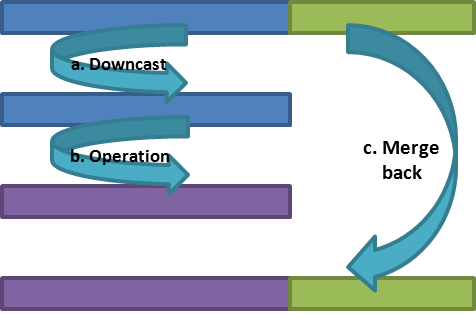
\psfig{file=heap_upcasting.png,height=5cm}} \caption{Coercing references.\label{fig:ref_coerce}}
\end{figure}

We instance the coercion predicate for references to perform a single step of coercion, that is for the case when we have a reference to a memory $tl$ and we want to use it where we expect a memory $Cons\ h\ tl$:
\begin{lstlisting}
class HList tl => Coercible (Ref tl a) (Ref (Cons h tl) a) where
  coerce ref =
    Ref (ST(\(Cons h tl) ->
      let (tl$'$,res) = get ref tl
      in (h $'$Cons$'$ tl$'$, res))
        (\v -> ST(\(Cons h tl) -> 
          let (tl$'$,()) = set ref tl v
          in (h $'$Cons$'$ tl$'$, ())))
  where get (Reference (ST g) _) = g
    set (Reference _ s) = \st -> \v -> 
      let (ST s$'$) = s v
      in s$'$ st
\end{lstlisting}

Now we can finally rewrite the example above to make use of our new coercion operator:
\begin{lstlisting}
ex3 :: ST Nil Unit
ex3 = do+ i <- new 10 :: Ref (New Nil Int) Int
          s <- new "Hello" :: Ref (New (New Nil Int) String) String
          (coerce i) *= (+2)
          s *= (++" World")
          return ())
\end{lstlisting}
 

\section{Objects}
\label{sec:objects}
\section{Objects}
We now start with the characterization of objects in our system. The $Object$ predicate says that an object will be a record which supports methods and inheritance; of course all the object operators are expected to work in conjunction with the rest of the system. Since objects will reference themselves, to avoid recursive type definitions we give a predicate that allows us to freely add or remove some constructor from an object:
\begin{lstlisting}
class Recursive o where
  type Rec o :: *
  to :: o -> Rec o
  from :: Rec o -> o
\end{lstlisting}

An object is required to support the $Recursive$ predicate:
\begin{lstlisting}
class (Record o st s, Recursive o, ro~Rec o) => Object o st s where
  type Base o :: *
  get_base :: Ref st s o -> Ref st s (Base o)

  type Method ro st :: * -> * -> *
  (<=|) :: Ref st s r -> Label r (Method ro st a b) -> a -> st s b
\end{lstlisting}

With respect to inheritance, it looks clear how we can instance coercion to take advantage (and make access more uniform) of the $base$ operations:
\begin{lstlisting}
instance Object o st s => Coercible (Ref st s o) (Ref st s (Base o)) where
  coerce = get_base
\end{lstlisting}

We also add a further predicate that characterizes inheritance:
\begin{lstlisting}
class Inherits a b

instance (Object o st s) => Inherits o (Base o)
\end{lstlisting}

Notice that methods are defined with a different operator than the selection operator for records. This can be addressed as follows: we define a new predicate for selecting something from a reference through a label:
\begin{lstlisting}
class Selectable st t s a where
  type Selection s t a :: *
  (<=) :: Ref st s t -> Label t a -> Selection s t a
\end{lstlisting}

We instance this predicate twice, one for field selection and one for method selection. Before doing so, though, we must be careful to disambiguate the last parameter in the record definition. For this purpose we add a $Field$ type function that represents a placeholder type that will distinguish fields from methods and inherited types:
\begin{lstlisting}
class (RefSt st s) => Record r st s where
  type Label r :: * -> *
  type FieldSlot a :: *
  (<==) :: Ref st s r -> Label r (FieldSlot a) -> Ref st s a
\end{lstlisting}

In the case of simple mutable records we can easily add a trivial constructor for $FieldSlot$ such as:
\begin{lstlisting}
data Field a = Field a
\end{lstlisting}

Now we can instance the selection predicate:
\begin{lstlisting}
instance Record st r s => Selectable st r s (FieldSlot a) where
  type Selection s r (Field a) = Ref st s a
  (<=) = (<==)

instance (Object st o s, ro~Rec o) => Selectable st o s (Method ro a b) where
  type Selection s o (Method ro a b) = a -> st s b
  (<=) = (<=|)
\end{lstlisting}

The final operation we wish to support is that of selecting a method or a field directly from any of the inherited classes of an object without explicit coercions:
\begin{lstlisting}
instance (Object st o s, bo~Base o, Selectable st bo s a) => Selectable st o s a where
  type Selection s o a = Selection s bo a
  (<=) = get_base . (<=)
\end{lstlisting} 

\section{Mutable Objects}
\label{sec:mutable_objects}
\section{Mutable Objects}
We now implement mutable objects. We start with inheritance:
\begin{lstlisting}
data Inherit x = Inherit x

instance (o ~ (BaseCons bo 'Cons' no), Record o ST s => Object o ST s where
  type Base o = bo
  get_base self_ref =
	StRef(do ((BaseCons base) 'Cons' tl) <- eval self_ref
           return base)
       (\base' -> do (_ 'Cons' tl) <- eval self_ref
           self_ref := ((Inherit base') 'Cons' tl)
           return ())

  ...

instance (o ~ (Unit 'Cons' so), Record o ST s => Object o ST s where
  type Base o = o
  get_base self_ref = self_ref

  ...
\end{lstlisting}
In our mutable encoding the first field of the object must be either the value of the inherited value or unit when the object does not inherit anything.

Methods enjoy the same implementation in both cases, so we just give one:
\begin{lstlisting}
data MethodCons t a b = MethodCons(t -> a -> (b,t))

instance (o ~ (Unit 'Cons' so), Record o ST s => Object o ST s where
  ...

  type Method ro st a b = MethodCons ro a b
  self_ref <=| (Label read write) = 
             \x -> do self <- eval self_ref
                      let (MethodCons m) = read self
                          (res,self') = m self x
                      self_ref := self'
                      return res
\end{lstlisting}

It can prove very useful to take advantage of our existing infrastructure to create methods from references and statements, so that the user of our system will not be forced to define methods by explicitly tracking mutations to the value of $this$; for this reason we add a function to the $Object$ predicate that converts a method from reference to state into our format (the implementation here is the same for both instances of $Object$, so we provide only one:
\begin{lstlisting}
class (Record o st s, Recursive o, ro~Rec o) => Object o st s where
  ...
  mk_method :: (StRef o o -> a -> st o b) -> Method ro st a b

instance (o ~ (Unit 'Cons' so), Record o ST s => Object o ST s where
  ...
  mk_method m = Method(\this->\args->
                         let (ST res_st) = m state_ref args
                         in res_st this)
\end{lstlisting} 

\section{Sample: Vectors}
\label{sec:vectors}
We now implement a simple example that shows how we can define a system of mutable vectors.

We begin by defining a 2d vector ($Vector2$) with two methods and a 3d vector ($Vector3$) with two other methods and which inherits the 2d vector:
\begin{lstlisting}
type Vector2Def k = Field St Float `Malloc` Field St Float `Malloc` Method St k () () `Malloc` Method St k () Float `Malloc` Nil
data RecVector2 = RecVector2 (Vector2Def RecVector2)
type Vector2 = Vector2Def RecVector2
instance Recursive Vector2 where
  type Rec Vector2 = RecVector2
  to = RecVector2
  from (RecVector2 v) = v
x :: Label St Vector2 (Field St Float)
x = labelAt Z
y :: Label St Vector2 (Field St Float)
y = labelAt (S Z)
norm2 :: Label St Vector2 (Method St (Rec Vector2) () ())
norm2 = labelAt (S (S Z))
len2 :: Label St Vector2 (Method St (Rec Vector2) () Float)
len2 = labelAt (S (S (S Z)))

mk_vector2 :: Float -> Float -> Vector2
mk_vector2 xv yv = (StField xv) `Malloc` (StField yv) `Malloc` norm `Malloc` len `Malloc` Nil
                    where norm = mk_method (\this -> \() -> do l <- (this <= len2) ()
                                                               (this <= x) *= (/ l)
                                                               (this <= y) *= (/ l))
                          len = mk_method (\this -> \() -> do xv <- eval (this <= x)
                                                              yv <- eval (this <= y)
                                                              return (sqrt(xv * xv + yv * yv)))

type Vector3Def k = Inherit Vector2 `Malloc` Field St Float `Malloc` Method St k () () `Malloc` Method St k () Float `Malloc` Nil
data RecVector3 = RecVector3 (Vector3Def RecVector3)
type Vector3 = Vector3Def RecVector3
instance Recursive Vector3 where
  type Rec Vector3 = RecVector3
  to = RecVector3
  from (RecVector3 v) = v
z :: Label St Vector3 (Field St Float)
z = labelAt (S Z)
norm3 :: Label St Vector3 (Method St (Rec Vector3) () ())
norm3 = labelAt (S (S Z))
len3 :: Label St Vector3 (Method St (Rec Vector3) () Float)
len3 = labelAt (S (S (S Z)))

mk_vector3 :: Float -> Float -> Float -> Vector3
mk_vector3 xv yv zv = StInherit (mk_vector2 xv yv) `Malloc` StField zv `Malloc` norm `Malloc` len `Malloc` Nil
                      where norm = mk_method (\this -> \() -> do l <- (this <= len3) ()
                                                                 ((get_base this) <= x) *= (/l)
                                                                 ((get_base this) <= y) *= (/l)
                                                                 (this <= z) *= (/l)) 
                            len = mk_method (\this -> \() -> do xv <- eval ((get_base this) <= x)
                                                                yv <- eval ((get_base this) <= y)
                                                                zv <- eval (this <= z)
                                                                return (sqrt(xv * xv + yv * yv + zv * zv)))

ex4 :: forall mem . mem ~ (Vector3 `Malloc` Nil) => St Nil Nil Bool
ex4 = do+ v <- new (mk_vector3 0.0 2.0 (-1.0))
          xv <- eval ((get_base v) <= x)
          let v' = coerce v :: Ref St mem Vector2
          xv' <- eval (v' <= x)
          (v' <= norm2)()
          (v <= norm3)()
          return (xv == xv')
          delete

res4 :: Bool
res4 = runSt ex4 Nil
\end{lstlisting}

where we expect that $res=True$. Notice how select labels that are defined for a 2d vector on an instance of a 3d vector, and how we access the same label on the value of $base$ obtained through coercion on the 3d vector.
 

\section{Alternate Implementations}
\label{sec:alternate}
\section{Alternate Implementation}
In the following sections we give alternate implementations of our system. We do so in order to exploit its flexibility by showing how the same primitives allow us to define very different execution models:
\begin{itemize}
\item A transactional model
\item A concurrent/distributed model
\item A reactive model
\end{itemize}

Each model is characterized by a predicate that expresses some requirements on its state, reference or stack types so as to allow different implementations of the same model (for example to experiment with faster algorithms, etc).

The predicate for the transactional model simply states that there must be three methods for opening, closing and undoing transactions. Notice that transactions might also be used for implementing undo buffers in a very simple and clean way:
\begin{lstlisting}
class Transactional st where
  beginT :: st s ()
  commitT :: st s ()
  abortT :: st s ()
\end{lstlisting}

The predicate for concurrency requires a method for forking computations:
\begin{lstlisting}
class Concurrent st where
  fork :: (st s (), st s ()) -> st s ()
\end{lstlisting}

The reactive model has no specific requirements, and is simply an alternate instantiation of the object system typeclasses.

In addition to these three implementations, we will discuss a system for reflection on objects. Reflective objects will validate a predicate ($ReflectiveObject$) which allows to obtain the labels that respect certain conditions; being labels first class objects, they will then be passed around and used freely for selection on objects of the appropriate type:
\begin{lstlisting}
class (Object o ref st s, ro~Rec o) => ReflectiveObject o ref st s where
  get_fields :: [Label o (Field a)]
  get_methods :: [Label o (Method ro a b)]
\end{lstlisting}
 

\end{document}
